\documentclass{standalone}

\usepackage{tikz}

\begin{document}
\Large
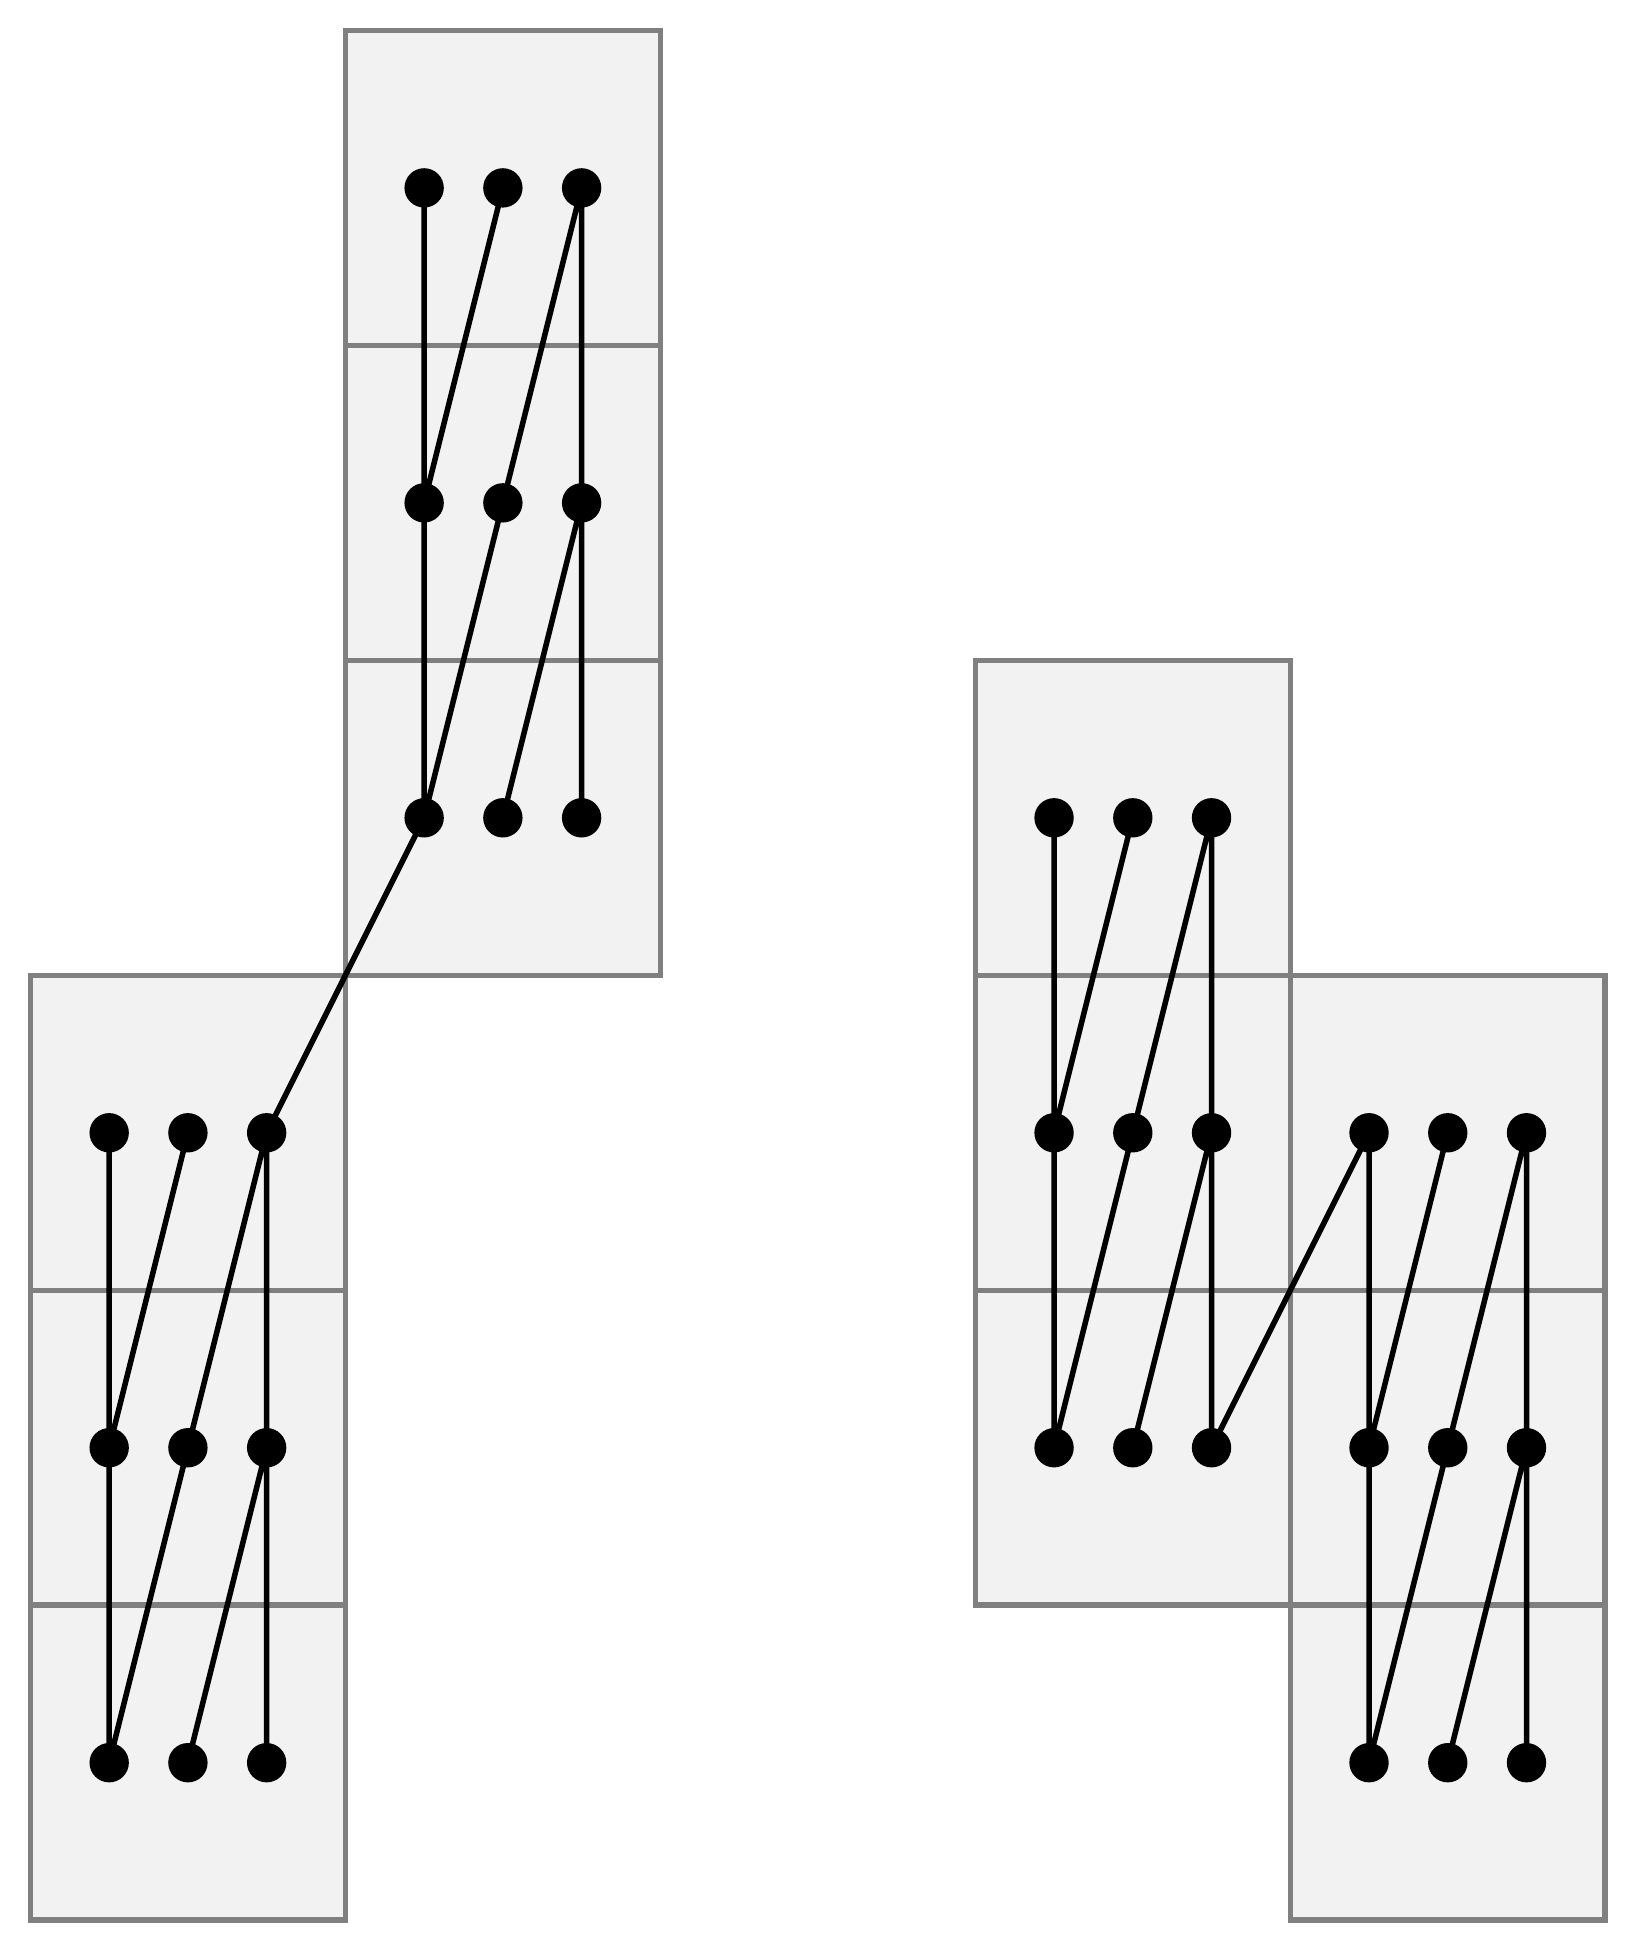
\begin{tikzpicture}
% \draw[help lines, black!30] (0,0) grid (12,12);
\foreach \a in 
    {(0,0), (0,4), (0,8), (4,12), (4,16), (4,20),
     (16,0), (16,4), (16,8), (12,8), (12,12), (12,4)}
    {\draw[line width=0.7mm, black!50, fill=black!5] \a rectangle ++(4,4);
    \fill 
        \a++(1,2) circle (0.25)
        \a++(2,2) circle (0.25)
        \a++(3,2) circle (0.25);
        };
\foreach \a in 
    {(0,0), (0,4), (4,12), (4,16), (16,0), (16,4), (12,8), (12,4)}
    {\draw[line width=0.7mm]
        \a++(1,2) -- ++(0,4)
        \a++(1,2) -- ++(1,4)
        \a++(2,2) -- ++(1,4)
        \a++(3,2) -- ++(0,4);
    };
\draw[line width=0.7mm]
        (3,10) -- (5,14)
        (17,10) -- (15,6);
\end{tikzpicture}
\end{document}